%\addbibresource{/home/jorgsk/phdproject/bibtex/jorgsk.bib}
The paper by Kucharova et al.\ on page \pageref{vero_paper} deals with gene
expression systems in bacteria and how these systems are regulated by codon
usage bias, mRNA stability, and RNA secondary structures at the ribosome
binding site (RBS). Here, we review each of these topics. We begin with a brief
account of translation initiation and then talk about how this process is
regulated by RNA secondary structures. We then proceed to translation
elongation and how this process is affected by condon usage bias.

\subsubsection{Brief overview of translation}
Translation is the conversion of the genetic code of an mRNA into an amino acid
sequence. The molecule responsible for this is the ribosome, a macromolecular
complex of RNA and protein. The ribosome consists of two subunits, S30 and S50,
which initiate translation by binding sequentially (first S30, then S50) close
to a start codon in the 5\ppp region of an mRNA.  Together, they read the
genetic code in the form of nucleotide triplets (e.g.\ AAG) called codons. Each
codon is matched with an anticodon in a transfer RNA (tRNA) which carries the
amino acid that corresponds to this codon. The amino acids from the tRNAs are
joined to each other in the ribosome to form the primary protein sequence which
eventually will fold into a sequence specific conformation.

Since bacteria have no nucleus, the ribosome can bind the 5\ppp-end of an mRNA
at the same time as the mRNA is being synthesized. The coupling of translation
with transcription is called co-transcriptional translation. The first ribosome
that initiates translation on an mRNA follows the transcribing RNA polymerase
closely and even pushes it, causing both of them to follow the same speed
\cite{proshkin_cooperation_2010}. In this way, the ribosome can prevent RNAP
from backtracking, which can increase the speed of transcription by reducing
RNAP pausing. Fascinatingly, it was recently shown that by preventing RNAP
backtracking in this way, ribosomes reduce collisions between RNAP and DNA
polymerases during chromosome duplication, and that reducing these collisions
leads to fewer errors during genome duplication \cite{dutta_linking_2011}. This
links the seemingly disparate topics of translation and genome integrity and is
an example of the interconnectedness of the cell.

\subsubsection{Translation initiation: binding of the 16S RNA to the
Shine-Dalgarno sequence}
The 16S RNA is a ribosomal RNA which is part of the S30 ribosome subunit and is
important for translation initiation. It was shown by Shine and Dalgarno in
1974 that the last nine bases of the 3\ppp end of the 16S RNA in \textit{E.
coli} are ACCUCCUUA \cite{shine_3-terminal_1974}. They suggested that this
sequence could hybridize to a previously discovered conserved complementary
motif close to the start codon in the 5\ppp untranslated region (UTR) of mRNA,
and that this hybridization facilitated the initiation of translation
\cite{shine_3-terminal_1974}. That this actually occurs was later confirmed and
it is now known to be the canonical method of translation initiation in
prokaryotes (bacteria and archaea) \cite{nakagawa_dynamic_2010}. Examples of
translation initiation occurring without 16S RNA hybridization have been found,
but they are exceptions rather than the rule \cite{skorski_highly_2006,
boni_non-canonical_2001}.

The complementary motif on mRNA that 16S RNA hybridizes to is known as the
Shine-Dalgarno sequence, and the complementary bases on 16S RNA is known as the
anti Shine-Dalgarno sequence. The Shine-Dalgarno (SD) sequence is located 3 to
10 bases upstream the start codon. Its sequence is often given as GGAGGA
although the core motif can be reduced to GGAG. This sequence and its position
relative to the start codon are conserved across prokaryotes with very little
variation \cite{nakagawa_dynamic_2010}. 

When the 16S RNA hybridizes with the SD sequence during translation initiation,
the S30 subunit becomes physically anchored to the transcript. The binding of
the S30 subunit facilitates the binding of the S50 subunit, which completes the
binging of the ribosome to mRNA. The ribosome now covers an area +/- 15 nt
around the start codon; this area is called the ribosome binding site (RBS)
\cite{kozak_regulation_2005} (see Figure \ref{fig:translation_initiation}).
When the 30S subunit binds the SD sequence, the start codon on mRNA (mostly AUG
in \textit{E. coli}) becomes aligned to the peptidyl site on S30. This allows
the first initiating tRNA to bind and begin amino acid chain synthesis.
\begin{figure}[htb]
	\begin{center}
		\includegraphics[scale=1]{illustrations/translation_initiation.pdf}
	\end{center}
	\caption{Translation initiation. The 30S subunit binds the Shine-Dalgarno
	sequence, upon which the 50S subunit binds the 30S subunit to form the full
	ribosome. The bound ribosome occupies the ribosome binding site around the
	start codon.}
	\label{fig:translation_initiation}
\end{figure}

Since the SD sequence must basepair with 16S RNA, transcription initiation is
regulated by having the SD sequence basepair with another RNA sequence before
16S RNA can bind. There are two main types of RNA that bind the SD sequence to
block translation initiation. One type are trans-acting factors like microRNAs
\cite{storz_controlling_2004}. However, the most common source of RNA that
binds the SD sequence is cis-acting RNA from the same mRNA molecule that the
ribosome is binding to. Cis-acting RNA can bind to the SD if a sequence on the
mRNA is complementary to the SD sequence (Figure \ref{fig:hairpin_blockage}).
This type of RNA folding is a potent regulator of transcription initiation
\cite{hall_role_1982, de_smit_secondary_1990}, and will now be covered in more
detail.

\begin{figure}[h]
	\begin{center}
		\includegraphics[scale=0.5]{illustrations/hairpin_blockage.pdf}
	\end{center}
	\caption{Binding of the ribosome to mRNA can be blocked if a secondary
	structure is formed using the SD sequence.}
	\label{fig:hairpin_blockage}
\end{figure}

\subsubsection{Co-transcriptional RNA folding}
To understand how the folding of RNA in the RBS affects translation initiation,
it is necessary to understand how the folding of mRNA occurs in general. The
basis for RNA folding is that RNA, as DNA, can basepair with itself; C pairs
with G and A pairs with U. The reason why RNA folds under physiological
conditions is that base-paired nucleotides are more thermodynamically favorable
than free nucleotides \cite{onoa_rna_2004}. Folded RNA is often depicted as a
series of so called hairpins with base-paired stems and loops on top. Hairpins
are examples of RNA secondary structures. More complex tertiary RNA structures
can also form by the hybridization of secondary structures. However, tertiary
structures form more slowly than secondary structures \cite{onoa_rna_2004}, and
are therefore not as relevant in obstructing ribosome binding.

As the nascent RNA emerges from the RNA exit channel of bacterial RNAP it is
immediately free to fold into an energetically favorable conformation. The
folding of the mRNA at the same time as it is being transcribed is called
co-transcriptional folding. A key question in co-transcriptional RNA folding
has been how comparable the time scales for RNA folding and RNA synthesis are
\cite{de_smit_translational_2003}. The degree of RNA co-transcriptional folding
depends on the timescale for folding relative to the time scale for RNA
synthesis. In bacteria, RNA synthesis happens at a rate of between 20 and 80 ms
per nucleotide, while formation and dissociation of semi-stable structures like
helices occur on the 10 to 100 $\mu$s timescale \cite{isambert_jerky_2009}. In
other words, for each nucleotide synthesized, there is on average time for 1000
refolding events. It should however be noted that the time needed for the
spontaneous refolding of an RNA structure depends on binding strength of
that structure; only relatively weak structures can be expected to change
during co-transcriptional folding.

The exact order of folding steps the mRNA undergoes as it is synthesized is
called the RNA's folding pathway. It is assumed that the folding pathway of an
RNA is under selective pressure to either ensure or prevent that certain
transient or permanent secondary structures are formed\cite{pan_rna_2006}. An
example of such selection could be a folding pathway that avoids secondary
structures in the RBS, which could be the result of a selective pressure for a
high translation initiation rate at this RBS.

\subsubsection{RNA secondary structures in the ribosome binding site}
It was shown already in the early 80s that translation rates are strongly
affected by secondary structures at the RBS \cite{hall_role_1982}. In a seminal
study, Smit and Duin modified both the location and the binding strength of
secondary structures in the RBS of an mRNA to find that the level of the
expressed protein could be varied over 500 fold
\cite{de_smit_secondary_1990}. They concluded that this reflected a variation
in the efficiencies of translation initiation on the mRNA caused by these
changes. In particular, they found a non-linear relationship between the
folding energy of structures in the RBS and the translation initiation rate:
above a certain threshold, the translation initiation rate did not change with
respect to the strength of the secondary structure; but below that limit,
translation initiation decreased exponentially as the secondary structures in
the RBS got stronger \cite{de_smit_secondary_1990}.

In general, it is thought that the entire RBS sequence must be unstructured for
translation initiation to occur \cite{seo_quantitative_2009}. It is therefore
not surprising that the absence of strong secondary structures is a hallmark of
ribosome binding sites in several species \cite{gu_universal_2010}. The folding
energy of the RBS in the \textit{E. coli} transcriptome can even be used to
distinguish between active genes and pseudogenes \cite{keller_reduced_2012}.
This may be because pseudogenes are no longer under selective pressure
to avoid strong secondary structures in the RBS as they no longer code for
functional proteins and therefore do not need to be translated by ribosomes
\cite{keller_reduced_2012}.

It should be noted that although the RBS is generally void of strong secondary
structures, there are many examples of structured ribosome binding sites
\cite{studer_unfolding_2006}. To account for how the ribosome would bind to
mRNA with structures in the RBS, it was initially suggested that the ribosomes
would only bind when the structures in the RBS spontaneously unfolded
\cite{de_smit_translational_1994}. However, it was later appreciated that the
time scale for RNA folding and unfolding are orders of magnitude faster than
the time scale for ribosome binding to RNA. This led to the suggestion that
ribosomes could first bind to a so called ribosome standby site close to the
RBS from where they could approach the RBS when the secondary structures there
unfolded \cite{de_smit_translational_2003}. This has however not been
conclusively demonstrated, but was partially supported by a study that showed
that that the ribosome, together with translation initiation factors, may
unwind secondary structures at the RBS presumably from ribosome standby sites
\cite{studer_unfolding_2006}.

\subsubsection{Modifying the RBS to increase gene expression}
As previously mentioned, it has been known since the early 80s that nucleotide
substitutions in the RBS can affect gene expression
\cite{warburton_increased_1983}. This is obvious for the SD sequence and the
start codon, since these sequences must be bound by complementary sequences in
16S RNA and the initiating tRNA, respectively.  However, mutations outside
these elements may also affect gene expression, primarily by modifying the RNA
secondary structure around the RBS \cite{park_design_2007,
care_translation_2007}. If mutations in the RBS are introduced upstream the start
codon in the 5\ppp UTR, secondary structures in the RBS may be altered with the
advantage of not having to modifying the peptide sequence. An alternative is to
make synonymous codon changes in the first codons of a gene
\cite{cebe_rapid_2006}, which also will leave the amino acid sequence intact.

A different approach than mutagenizing the RBS to modify expression is to introduce
a new RBS in the form of a 5\ppp fusion partner \cite{lavallie_gene_1995}. The
fusion partner is usually the 5\ppp-end (5\ppp UTR and early coding region) of
a gene that is already known to be well expressed in the host organism or has
other useful properties (such as the His-tag for protein purification
\cite{cebe_rapid_2006}). When using a 5\ppp fusion partner the peptide coded by
the early coding region of the fusion partner will be added to the N-terminus
of the protein that is being expressed. This fusion peptide may later be
cleaved off by specific proteases or left in place if its presence is tolerated
\cite{esposito_enhancement_2006}.

When one wants to optimize the expression of a given gene, one may turn to
commercial providers of gene optimization, such as DNA 2.0 or GenScript.
However, there are published alternatives. In addition to what has been already
mentioned about fusion tags and RBS mutagenesis, the most comprehensive tool
yet published for optimization of translation initiation is the RBS calculator
\cite{salis_automated_2009}. This software takes into account several sequence
dependent variables that have been shown to play a role in translation
initiation: the match of the 16S RNA to the SD sequence, the distance from the
SD sequence to the start codon, the folding energy of any RBS secondary
structures, the type of start codon, and the folding energy of the ribosome
standby site \cite{salis_automated_2009}. Given an input mRNA sequence centered
around the start codon, the tool will suggest sequence changes that will result
in a calculated optimal translation initiation rate for the gene of interest.

%\subsubsection{RNA secondary structures affect RNA stability}
%RNA secondary structures do not only affect ribosome binding, but they also
%affect the stability of RNA. RNA stability is a term used to describe the
%half-life of RNA in the cell; it is a measure of how long it takes from an RNA
%is produced until it is degraded. If all else is equal, a stable transcript
%would result in more protein being produced from it than an unstable
%transcript. As well, after an mRNA is produced from a gene, RNA degradation is
%the final way to stop protein expression from that gene. For these reasons, RNA
%stability is carefully regulated in the cell.

%There are two well-known ways in which RNA secondary structures affect RNA
%stability. The first is by hairpin structures at the 5\ppp and 3\ppp ends of
%the RNA. The effect of a hairpin at the 5\ppp-end of an RNA is that the hairpin
%protects the 5\ppp-most nucleotide in the RNA against attack from the protein
%RppH. RppH modifies 5\ppp nucleotides by removing a phosphate group
%\cite{deana_bacterial_2008}. If a 5\ppp nucleotide lacks this phosphate group,
%the whole RNA becomes a target for RNAse E, an endonuclease which
%can initiate RNA degradation \cite{mackie_ribonuclease_1998}. In this way, a
%5\ppp hairpin indirectly protects the mRNA against degradation by RNAse E. The
%function of the 3\ppp hairpin is more direct. It protects directly against
%degradation from RNAse which require RNA with an unstructured 3\ppp-end for
%their activity \cite{rauhut_mrna_1999}.

%The second way RNA structures affect RNA stability is through their already
%mentioned effect on ribosome binding. It is well established that actively
%translated mRNA are more stable than untranslated mRNA. This led to the idea
%that the narrow spacing between translating ribosomes on the transcript would
%prevented cleavage by RNAse \cite{deana_lost_2005}. However, it has been shown
%in at least two cases that ribosome binding confers transcript stability on its
%own in the absence of translation \cite{wagner_efficient_1994,
%hambraeus_5_2002}. This indicates that narrow spacing between translating
%ribosomes is not necessary for increased stability.  Therefore, the precise
%mechanism for how ribosome binding prevents degradation is not clear
%\cite{deana_lost_2005}.

\subsubsection{Codon bias affects gene expression and cellular fitness}
During translation elongation the ribosome matches incoming amino acids on
transfer RNAs (tRNA) to codons on the mRNA. There are 64 ($4^3$) codons present
in the genomes of nearly all organisms studied to date. Generally, 61 of these
match the anti-codons on tRNA and the remaining three are stop codons. On the
other hand there are only 20 amino acids carried by the 61 tRNA. The
explanation for this discrepancy is that several codons are associated with the
same amino acid. These codons are synonymous: they code for the same amino
acid. For example, the codons AAA and AAG both code for lycine.

Even though several codons can be synonymous, they are often found with
different frequencies in genomes. The preference of one synonymous codon over
another is called codon usage bias. Codon usage bias is a universal phenomenon
as it is found throughout the kingdom of life \cite{sharp_codon_1988}. In many
species, codon bias is especially strong in highly expressed genes, which seems
to indicate that the over-represented codons in these genes are especially
suited for high rates of translation.  This has led to the suggestion that some
codons are more ``efficient'' than others during translation and that genes
with efficient codons are translated more rapidly \cite{moriyama_gene_1998}. It
was eventually shown that the efficient codons are those that have the highest
copy numbers of the corresponding tRNA genes \cite{reis_solving_2004,
elf_selective_2003}. This seems to explain that efficient codons are translated
more rapidly because the corresponding tRNAs are more abundant in the cell,
shortening the waiting time between each tRNA binding event.

A commonly used measure for codon bias is the codon adaptation index (CAI). It
measures how similar a gene's codon content is compared to the codons in highly
expressed genes in the same organism \cite{sharp_codon_1987}. The CAI has
accordingly been shown to correlate positively with gene expression levels in
several species \cite{duret_expression_1999, jansen_revisiting_2003}. The CAI
has been used for codon optimization of genes for heterologous expression;
for example, codon optimization has been used to achieve high expression levels
when expressing human genes in bacterial hosts \cite{gustafsson_codon_2004}.
The underlying reason is that codon usage bias differs between species: a codon
which is rapidly translated in human may be slowly translated in \textit{E.
coli}.

Two recent publications have shed light on the effect that codon bias has on
the rate of translation. In the first, Kudla et al.\ made random synonymous
codons changes in the green fluorescent protein (GFP) gene to generate a
library of 154 GFP gene variants with on average 114 different codons each
\cite{kudla_coding-sequence_2009}. The GFP variants displayed a 250 fold
variation in expression in \textit{E. coli}, and caused a marked difference in
cell culture growth rates. The CAI of the GFP variants did in this study not
correlate with their expression levels, but instead, surprisingly, correlated
with the cell division rate of the cells. The expression level, on the other
hand, was found to correlated strongly with secondary structures around the
start codon, but did not show any correlation with cell growth rates. The
authors concluded from this that codon bias exists in highly expressed genes
not to optimize translation rates, but to optimize overall cellular fitness.
The hypothesis is that if highly expressed genes contained codons for which
there were few tRNA, ribosomes would often pause when translating the
corresponding mRNA, causing fewer ribosomes to be available to the rest of the
mRNA pool, thereby slowing the cellular growth rate
\cite{kudla_coding-sequence_2009}

In the second paper, Tuller et al.\ \cite{tuller_evolutionarily_2010} examined
the codon bias of 27 organisms from all three domains of life using the tRNA
adaptation index (tAI), a similar measure to the CAI. (Briefly, the tAI measure
ranks each codon with the gene copy number of the associated tRNA in the genome
\cite{tuller_evolutionarily_2010}). They found a species-wide trend where genes
tend to have inefficient codons in the early coding region (first 30-70
codons), but efficient codons in mid and late coding regions. The early
inefficient codons were labeled a slowly translated ``ramp''. Their hypothesis
is that by reducing the speed during early translation, ribosomes are more
evenly spaced out in the mid and late stages of translation elongation, which
reduces collisions between the ribosomes and thereby increases the overall
translation efficiency in the cell.

A criticism of the Tuller et al.\ paper is that the early codons of mRNA are
also under selective pressure to reduce mRNA folding \cite{gu_universal_2010}.
This would reduce the degrees of freedom for selection of optimal codons in the
early codon region, which could partly explain the ramp effect
\cite{plotkin_synonymous_2011}.

Finally, there are other sources of codon bias than have been mentioned so far.
One is the specific order that codons appear in, which has been linked to more
efficient recycling of tRNA \cite{cannarozzi_role_2010}. Another is the
avoidance of message-bearing motifs like the Shine-Dalgarno element in the
coding sequence. It was shown in \textit{E. coli} that when Gly-Gly amino acid
pairs are coded for in a gene, the most common codon pair is GGC-GGC, which out
of all possible Gly codon pairs has the lowest possible affinity for the
anti-Shine Dalgarno sequence. On the other hand, the rarest codon pair for
Gly-Gly was GGA-GGU, which is an exact match to the Shine-Dalgarno sequence
\cite{li_anti-shine-dalgarno_2012}. In the same study it was shown that
Shine-Dalgarno sequences inside coding regions could cause rebinding of the 16S
RNA during translation elongation and thereby cause translation pausing.
Interestingly, this rebinding behavior is the same as found for the sigma
factor during transcription elongation by RNA polymerase
\cite{mooney_sigma_2005}, as discussed on page \pageref{sigma_rebinding}. This
shows that the strong binding affinities of sigma for the promoter and 16S RNA
for the Shine-Dalgarno sequence can have the secondary effect where DNA
sequence in specific regions are selected on to avoid these signals.
